\scanpage{6}
\mspage{2}
% archive foliation: 5
Soit $G=\operatorname{End}(a)$, $\widehat A\simeq(G\text{-ens})$,
supposons $G=\{\operatorname{id}_a\}$, alors $\widehat A\simeq(\operatorname{Ens})$,
$\widehat A_{\mathrm{as}}=\text{Ens \unsure{uniponctuels}}$,
donc
\[
M_{\mathrm{as}}=\{x\in\operatorname{Ob}M\mid\operatorname{Hom}(a,x)\text{ card }1\}
\]
\deleted{donc} Contr'exemple: $M$ cat. discrète de cardinal $\geq2$, !

On \unsure{va supposer} que $M_{\mathrm{as}}$ engendre $M$ de façon que
\deleted{$\unsure{i^*}$ soit} $M\longrightarrow\widehat{M_{\mathrm{as}}}$
soit fidèle et conservatif.
\margin{\unsure{)}}

\figure{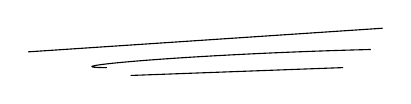
\begin{tikzpicture}[x=1cm,y=1cm]
\draw (0,.4)--(4.5,.7);
\draw (4.35,.43) .. controls (2,.37) and (.2,.2) .. (1,.2);
\draw (1.3,.1)--(4,.2);
\end{tikzpicture}}

\diagram{\begin{tikzcd}
\deleted{A}\arrow[r,hook]\arrow[rr,bend right=28] &
\deleted{M} & \deleted{M'}\arrow[l,"\deleted{f^*}"']
\end{tikzcd}}

\deleted{$f^*$ commute aux $\varprojlim$}

\deleted{$f_!$ existe alors, si on suppose que $\forall$ foncteur sur $M'$
qui commute aux $\varprojlim$ est représentable --- à vérifier des conditions
qui l'assurent, quitte parfois à faire des hyp. d'admissibilité sur $f^*$.
Mais va-t-on supposer que $f_!$ applique $M_{\mathrm{as}}$ dans $M'_{\mathrm{as}}$?}

\diagram{\begin{tikzcd}
\deleted{M}\arrow[r,shift left,"\deleted{f_!}"] &
\deleted{M'}\arrow[l,shift left,"\deleted{f^*}"]
\end{tikzcd}}

\deleted{Si $f:A\unsure{-|\longrightarrow} B$ asphérique, a-t-on
\[
f_!(\widehat A_{\mathrm{as}})\subset\widehat B_{\mathrm{as}}\ ?
\]
Par exemple prenons $B$ ponctuelle, \uline{$A$ cat. asph},}

\figure{\begin{tikzpicture}[x=1cm,y=1cm]
\draw (1.1,7.3) .. controls (1.5,4.6) and (3.2,1.2) .. (4.3,0.5);
\draw (4.8,7.3) .. controls (5.8,4.5) and (7.7,1.8) .. (7.6,1.2);
\draw (0,4.4) .. controls (.2,2.8) and (1.7,.4) .. (2.6,-.3);
\end{tikzpicture}}
